\documentclass[12pt,a4paper]{article}

% === PAQUETES === (((
\usepackage{amsmath}
\usepackage[shortlabels]{enumitem}
\usepackage{amsfonts}
\usepackage{ragged2e}
\usepackage{subfigure}
\usepackage{amssymb}
\usepackage{slashbox}
\usepackage{multirow}
\usepackage{multicol}
\usepackage{fontspec}
\usepackage{fullpage}
\usepackage{graphicx}
\usepackage{titlesec} 
% \usepackage{setspace}
\usepackage{dsfont}
% \usepackage{bookmark}
% )))

% === TIPOGRAFÍA === (((
\setmainfont[
  BoldFont       = bodonibi,
	ItalicFont     = Century modern italic2.ttf,
	BoldItalicFont = bodonibi,
	SmallCapsFont  = lmromancaps10-regular.otf
]{Century_modern.ttf}
% )))

% === COMANDOS === (((
\newcommand{\dis}{\displaystyle}
\newcommand{\qed}{\hspace{0.5cm}\rule{0.16cm}{0.4cm}}
\newcommand{\micita}[1]{\([\)\cite{#1}\(]\)}
\newcommand{\operator}[1]{\mathop{\vphantom{\sum}\mathchoice{ \vcenter{\hbox{\huge $#1$}} }
{\vcenter{ \hbox{\Large $#1$}} }{#1}{#1}}\displaylimits}
\newcommand{\suma}{\operator{ 
\includegraphics[scale=0.09]{IMAGENES/Sigma.png}} }
\DeclareSymbolFont{italics}{\encodingdefault}{\rmdefault}{m}{it}
\DeclareSymbolFontAlphabet{\mathit}{italics}
\ExplSyntaxOn
\int_step_inline:nnnn { `A } { 1 } { `Z }
 {  \exp_args:Nf \DeclareMathSymbol{\char_generate:nn{#1}{11}}{\mathalpha}{italics}{#1} }
\int_step_inline:nnnn { `a } { 1 } { `z } {  \exp_args:Nf \DeclareMathSymbol{\char_generate:nn{#1}{11}}{\mathalpha}{italics}{#1}}
\ExplSyntaxOff
% )))

% === SECCIONES === (((
\titleformat*{\section}{\large\normalfont\bfseries}
\titleformat*{\subsection}{\large\itshape \centering}
% \setcounter{secnumdepth}{0}
\renewcommand*{\contentsname}{\large\textbf{CONTENIDOS.}}
\usepackage[nottoc,numbib]{tocbibind}
\renewcommand{\refname}{REFERENCIAS.}
\renewcommand{\tablename}{Tabla}
\renewcommand{\figurename}{Figura}
% )))

% === PORTADA === (((
% \pagestyle{empty}
\newcommand{\portada}{
\addfontfeature{LetterSpace=-5}
  \begin{titlepage}
  \centering
  \begin{figure}
    \centering
    
\includegraphics[scale=0.5]{IMAGENES/logo_uaa.png}  
  \end{figure}
  {\bfseries\Large\MakeUppercase{\textit{Universidad Autónoma de Aguascalientes.}} \par}
  \vspace{1cm}
  {\Large Centro de Ciencias Básicas. \vspace{0.5cm}\\[2mm]
  Departamento de Matemáticas y Física.\vspace{0.5cm}\\[2mm]
  Licenciatura en Matemáticas Aplicadas.\vspace{0.5cm}\\[2mm]
  Práctica 6.\par}
  \vspace{1.5cm}
  {\bfseries\Huge Experimento de Young. \par} % title
  \vspace{1.5cm}
  {\itshape\Large Óptica. \\Prof. Mariana Alfaro Gómez.\par}
  % {\itshape\Large Variable Compleja I. \\Prof. Fausto Arturo Contreras Rosales.\par}
  % {\itshape\Large Métodos Numéricos II. \\Prof. Manuel Ramírez Aranda.\par}
  % {\itshape\Large Diseño de Experimentos. \\Prof. Angélica Hernández Quintero.\par}
  % {\itshape\Large Filosofía de la Investigación Científica. \\Prof. Jesús Mariano Rodríguez Muñoz.\par}
  \vfill
  % {\Large \textit{Por Erick I. Rodríguez Juárez.}\par}
		\begin{flushleft}
		\Large
		Alumnos:\\
		\textit{Carlos Francisco Guzmán Barba.}\\
		\textit{Erick Ignacio Rodríguez Juárez.}\\
		\textit{Manuel Alejandro Siller Landin.}
		\end{flushleft}
	% {}  % {\Large \textit{Por Erick I. Rodríguez Juárez.}\par}
  \vfill
		\begin{flushright}
		{\Large Realización: 2\(/\)05\(/\)22. \par} % date
		{\Large Entrega: 16\(/\)05\(/\)22. \par} % date
		\end{flushright}
  \end{titlepage} 
	% \thispagestyle{empty}
	% \doublespacing
	% \tableofcontents
	% \singlespacing
	% \newpage
} 
% )))

\begin{document}

\portada

\section{RESUMEN.} % (((
% )))

\section{INTRODUCCIÓN.} % (((

\subsection{--- Difracción en una Rendija Rectangular ---} % (((
\label{sub:difraccion_una}
\begin{figure}[hbtp!]
\addfontfeature{LetterSpace = -5}
\begin{minipage}{0.55\linewidth}
	\textbf{Definición.} \textit{En el movimiento de propagación de un sistema de ondas se le llama \textbf{difracción} al proceso experimental en el que chocan contra una pared con una abertura proporcional (rectangular , o circular) a la longitud de la onda.} \\[2mm]
 	En tal experimento, se tiene la siguiente situación.
	Las ondas que impactan la pantalla se relfejan detrás de ella.
	Aquellas que pasen por la abertura rectangular, se refractarán en todas las direcciones posibles, como lo indica la Figura \ref{fig:rectang} (tomada de \micita{hecht}).
\end{minipage}\hspace{5mm}
\begin{minipage}{0.45\linewidth}
	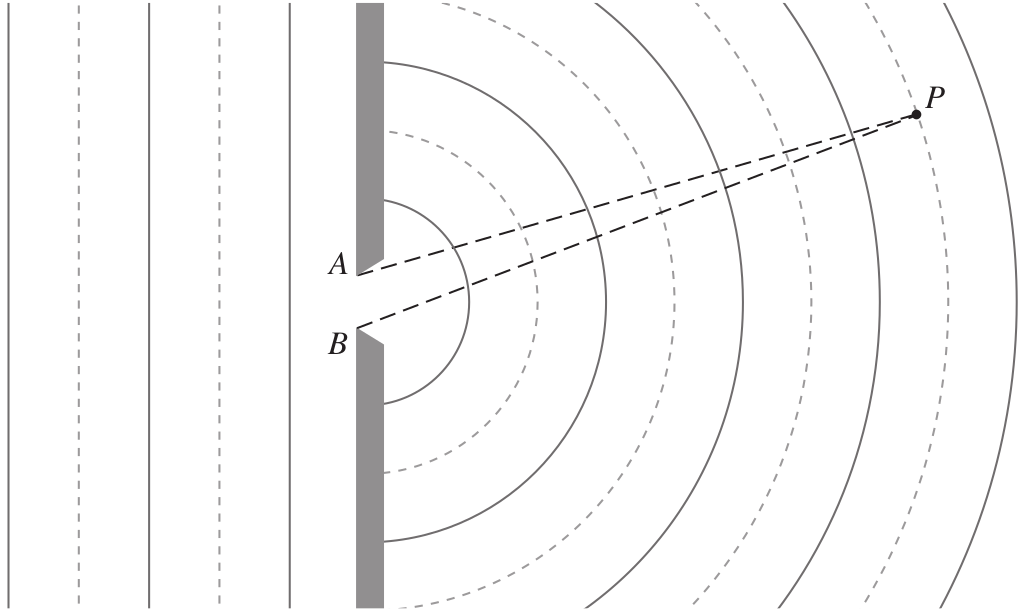
\includegraphics[width= 0.9 \linewidth]{1_INTRO/direcciones.png}
	\caption{Propagación de la onda.}
	\label{fig:rectang}
\end{minipage}
\end{figure}
\begin{figure}[hbt!]
	\addfontfeature{LetterSpace = -5}
	\begin{minipage}{0.4\linewidth}
	\centering
	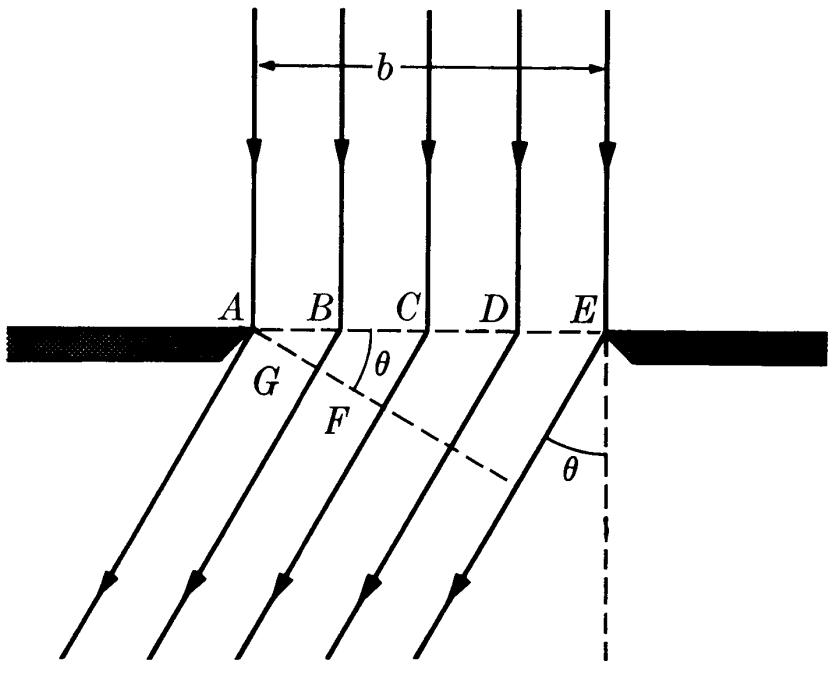
\includegraphics[width= \linewidth]{1_INTRO/seno.png}
	\caption{Difracción de la onda en la dirección del ángulo \(\theta\).}
	\label{fig:seno}
	\end{minipage}\hspace{5mm}
	\begin{minipage}{0.6\linewidth}
		Entonces las ondas que atraviesen la rendija alcanzarán un máximo en la onda, en aquellos ángulos \(\theta\), tal que las continuaciones de los rayos coincidan con los máximos antes de golpear la rendija. Como lo indica la Figura \ref{fig:seno} (obtenida de \micita{alonso_finn_1}).
		Es decir, si \(d\) es el tamaño de la rendija, \(\lambda\) la longitud de onda, y \(\theta\) el ángulo de desviación, tendremos:
		\begin{equation}
			d \sin \theta = m \lambda , \hspace{1cm} m \in \mathds{Z}.
			\label{eq:posicion_angular}
		\end{equation}
	\end{minipage}
\end{figure}
\begin{figure}[hbtp!]
	\addfontfeature{LetterSpace = -5}
	\begin{minipage}{0.5\linewidth}
		Además, notamos que si 
		% el ángulo \(\theta\) es suficientemente pequeño,
		\(y\) es la distancia del máximo central al \(m-\)ésimo máximo de la ec. (\ref{eq:posicion_angular}), y \(D\) es la separación de una pantalla con la rendija, entonces se tendrá \(\sin \theta = \tan \theta\), y
		\begin{equation}
			\tan \theta = \dfrac{y}{D}.
			\label{eq:distan_rendija}
		\end{equation}
		Así, como lo indica la Figura \ref{fig:constructiva}. Combinando (\ref{eq:posicion_angular}) y (\ref{eq:distan_rendija}), obtenemos que
		\begin{equation}
			y = \dfrac{m \lambda D}{d} , \hspace{1cm} m \in \mathds{Z} .
			\label{eq:altura}
		\end{equation}
	\end{minipage}\hspace{5mm}
	\begin{minipage}{0.5\linewidth}
		\centering
		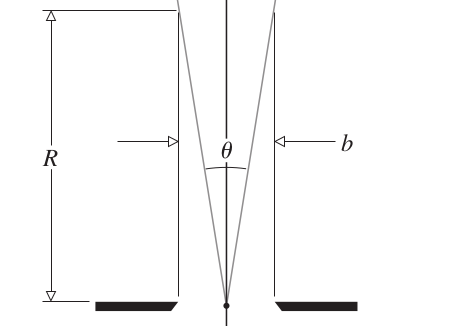
\includegraphics[width= 0.8 \linewidth]{1_INTRO/distancia}
		\caption{Tamaño de la difracción constructiva.}
		\label{fig:constructiva}
	\end{minipage}
\end{figure}
% )))

\subsection{--- Difracción de Doble Rendija ---} % (((
\label{sub:difraccion_dos}
Ahora, consideremos dos rendijas, ambas de tamaño \(a\), separadas a una distancia \(d\), como lo indica la Figura \ref{fig:exp_young}, al cual se le conoce como \textbf{Experimento de Young}.
\begin{figure}[hbt!]
	\centering
	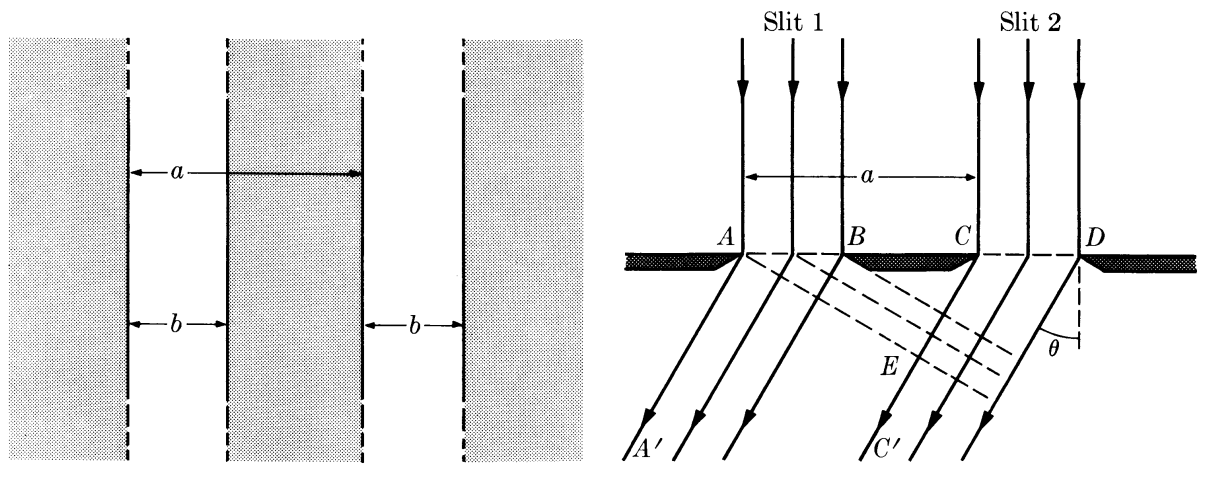
\includegraphics[width= 0.8 \linewidth]{1_INTRO/dos_rendijas.png}
	\caption{Experimento de Young.}
	\label{fig:exp_young}
\end{figure}\\
Notamos que la diferencia de fase entre ambas ondas es de
\[
	\alpha = \dfrac{2 \pi}{\lambda} CE = \dfrac{2 \pi d \sin \theta}{\lambda}.
\]
\begin{figure}[hbtp!]
	\addfontfeature{LetterSpace = -5}
	\begin{minipage}{0.5\linewidth}
	Notamos que, para la difracción de Faunhofer, se tiene la situación de la Figura \ref{fig:radios}. \\[2mm]
	Entonces, \(r \approx R - y \sin \theta\), y por cada rendija se tiene que 
		\[
			F(y) = \sin (wt- kr) = \sin (wt-k(R - y \sin \theta))
		\]
		Y también, para cada rendija tendremos la siguiente expresión para el campo eléctrico,
		\[
			E = C \dis\int _{y_{min}} ^{y_{max}} F(y) dy.
		\]
		Indicando que, en nuestro caso con dos rendijas, y con las longitudes de la Figura \ref{fig:exp_young}, obtendremos que
	\end{minipage}\hspace{5mm}
	\begin{minipage}{0.5\linewidth}
	\centering
	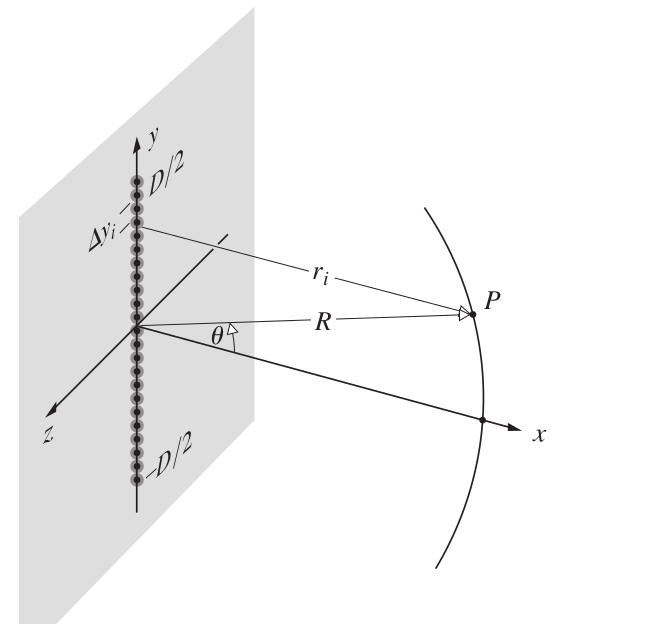
\includegraphics[width= 0.8 \linewidth]{1_INTRO/fran}
	\caption{Radios hacia la rendija.}
	\label{fig:radios}
	\end{minipage}
\end{figure}
\begin{equation}
	\begin{array}{rcl}
		E & = & C \dis\int _{-a/2} ^{a/2} F(y) dy + C \dis\int _{d-a/2} ^{d+a/2}  \\[5mm]
		& = & bc \bigg(\dfrac{\sin \beta}{\beta}\bigg) \big(\sin (wt-kR) + \sin (wt-kR + \alpha)\big)
	\end{array}
	\label{eq:campo_electrico}
\end{equation}
donde \(\beta = \dfrac{kb}{2} \sin \theta\), y \(\alpha = \dfrac{ka}{2} \sin \theta\). La gráfica de ésta función se deja indicada en la Figura \ref{fig:grafica}. 
\begin{figure}[hbt!]
	\centering
	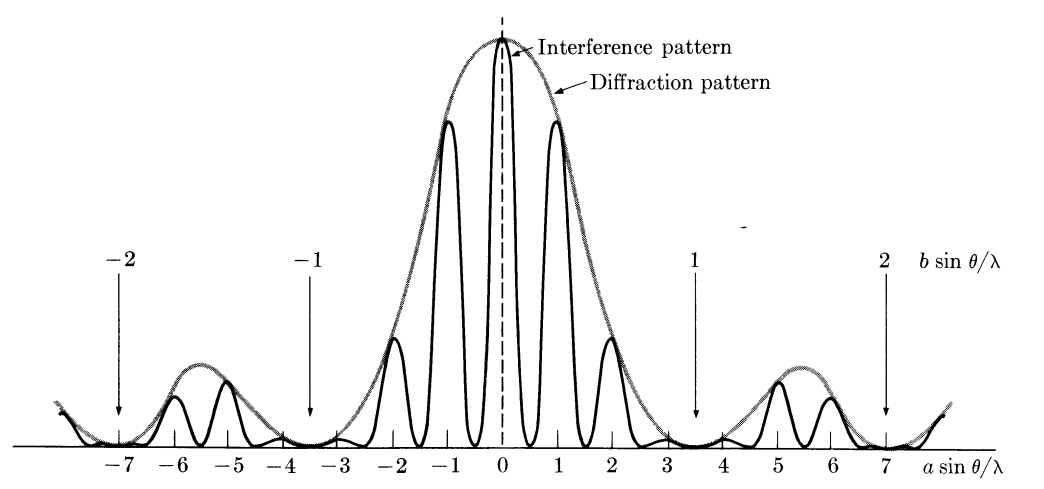
\includegraphics[width= 0.7 \linewidth]{1_INTRO/grafica}
	\caption{Gráfica de la función (4).}
	\label{fig:grafica}
\end{figure}\\
Además, se tiene \(I= \langle E \rangle ^2/2 = 4I_0 \bigg(\dfrac{\sin ^2 \beta}{\beta ^2}\bigg) \cos ^2\alpha \), se le llama irradiancia ``normalizada'' a la función \(I/(4I_0)\).
% )))

% )))

\section{METODOLOGÍA.} % (((
% )))

\section{RESULTADOS.} % (((
% )))

\section{DISCUSIÓN DE RESULTADOS Y CONCLUSIONES.} % (((
% )))

% === REFERENCIAS === (((
\bibliography{Referencias}
\bibliographystyle{unsrt}
% )))

\section{APÉNDICE.} % (((
% )))

\end{document}
